\UseRawInputEncoding
\documentclass[12pt]{report}
\usepackage{fullpage}
\usepackage{indentfirst}
\usepackage{verbatim}
\usepackage{gensymb}
\usepackage{amsthm}
\usepackage{amsmath}
\usepackage{graphicx}
\graphicspath{ {./images/} }
\usepackage{float}
\usepackage{subcaption}
\usepackage[title]{appendix}
\usepackage{listings}
\captionsetup{font=footnotesize}
\usepackage[cache=false]{minted}
\usepackage{multirow}
\usepackage{listings}

\theoremstyle{definition}
\newtheorem{exmp}{Example}[section]
\newcommand{\degrees}{\degree C }

\author{ISYE-6739 - Statistical Methods \\\\ Kadhir Umasankar}
\title{``Coins in a Pot" Simulation}
\date{December 7th, 2021}
\renewcommand\thesection{\arabic{section}}

\begin{document}
\maketitle

\begin{abstract}
Statistical analysis of games can be done by running many simulations. Statistics of interest can be recorded over many simulations, and when running thousands of such simulations, the estimations of statistics will begin to converge to the parameters' actual values. In this report, analysis of the ``Coins in a Pot" game will be described (the rules of this game will be explained in the report). The expected value and distribution of the number of cycles that the game will last for will be found. The process that was followed to write the Python code to simulate the game will be detailed. Plots of the distribution at various timesteps and the movement of the mean of the distribution over many simulations will be shown. Finally, the importance of writing code and simulating games as opposed to doing calculations by hand will be discussed.
\end{abstract}

\section{Introduction}

Analysis of games can be done by running many simulations. Code must be written to convert the problem at hand into a simulation that the computer can run, and statistics of interest can be recorded over many runs. By running thousands of such simulations, the estimates will begin to converge to the parameters' actual values, following the Law of Large Numbers, which can be seen in Equation \ref{eq:LLN}. The Law of Large Numbers says that ``the average of the results obtained from a large number of trials should be close to the expected value and will tend to become closer to the expected value as more trials are performed"\footnote{\texttt{https://en.wikipedia.org/wiki/Law\_of\_large\_numbers}}.

\begin{equation} \label{eq:LLN}
\bar{X_n} = \frac{1}{n}(X_1 + ... + X_n); \bar{X_n} \rightarrow \mu \text{ as } n \rightarrow \infty
\end{equation}

In this report, analysis of the ``Coins in a Pot" game will be described. In this game, two players start with 4 coins each, and the pot starts with 2 coins. The players take turns rolling a die, and they perform one of the following actions based on the number they roll:

\begin{table}[H]
\centering
\begin{tabular}{|c|l|}
\hline
\textbf{Number on Die} & \multicolumn{1}{c|}{\textbf{Action}}                     \\ \hline
1                      & Player does nothing                                      \\ \hline
2                      & Player takes all coins in the pot                        \\ \hline
3                      & Player takes half of the coins in the pot (rounded down) \\ \hline
4, 5, 6                & Player puts a coin in the pot                            \\ \hline
\end{tabular}
%\caption{Table of critical stress intensity factors ($K_C$) for different initial crack lengths ($a_0$)}
%\label{table:Dice}
\end{table}

The game ends when a player must put a coin in the pot but has no coins left. The number of cycles that the game lasts must be recorded, and its expected value and distribution are to be found.

Following these rules, some Python code was written to simulate the game. Section \ref{sim} of this report will discuss this code. The number of cycles that were played until a player ran out of coins was recorded in a list, and this process was repeated many times. The mean of the number of cycles will be found, and the distribution of the number of cycles will be plotted. Section \ref{results} will contain plots of the simulation, as well as a discussion of the results.

\newcommand{\code}[1]{\colorbox{lightgray}{\texttt{#1}}}

\section{Simulation Code}
\label{sim}

First, the logic of the game was coded in Python. A \code{Player} class was created to make it convenient to hold and handle transactions of coins between the players and the pot, and the two players and the pot were created as \code{Player} objects. A \code{for} loop was created, which would run iterations as specified by \code{num\_trials}. A nested \code{while} loop was created, which would run until a player had to put their coins into the pot but had none left. The number of cycles until the end of the game was recorded in a list, and the process was repeated. At the end of \code{num\_trials} iterations, the code plotted a histogram showing the distribution of the number of cycles, and calculated the mean of the distribution of cycles.

Some quality-of-life improvements were also made, such as using the \code{tqdm} package to show a progress bar as the code was performing iterations, and using \code{bashplotlib} to plot an ASCII version of the histogram in the command-line as the code was executing, an example of which can be seen in Figure \ref{fig:bashplot}. This code can be seen in the project's GitHub repository\footnote{\texttt{https://github.com/kadhirumasankar/isye-6739-project}}, as well as in Appendix \ref{pythoncode}.

\begin{figure}[H]
\centering
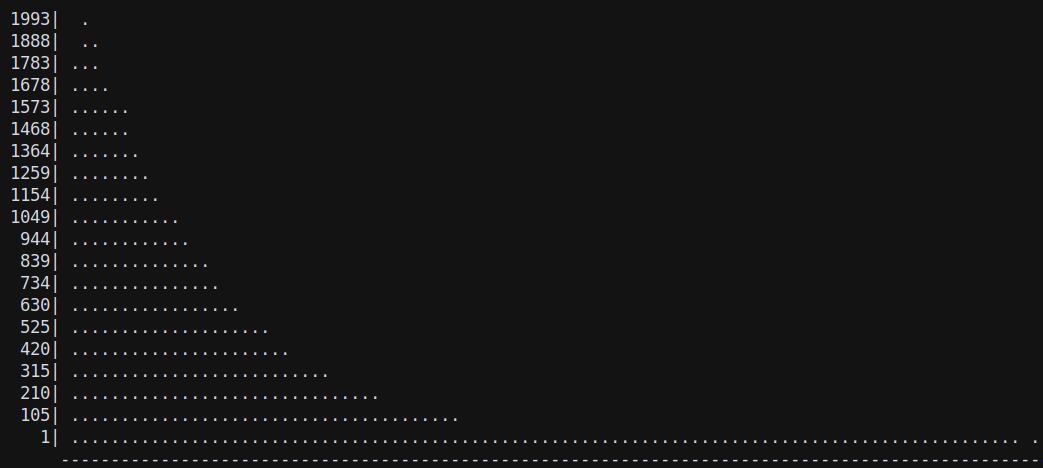
\includegraphics[width=.75\textwidth]{bashplot.png}
\caption{Screenshot of a histogram on the command-line, plotted using \code{bashplotlib}, to allow users to see changes in the distribution as the code is executing}
\label{fig:bashplot}
\end{figure}

\section{Results and Discussion}
\label{results}

Plots of the distribution of cycles after simulating 10, 100, 1,000, and 10,000 games can be seen in Figures \ref{fig:10} through \ref{fig:10000}. A plot of the distribution of cycles after simulating 1,000,000 games can be seen in Figure \ref{fig:1000000}.

\begin{figure}[H]
\centering
\begin{subfigure}{.4\textwidth}
  \centering
  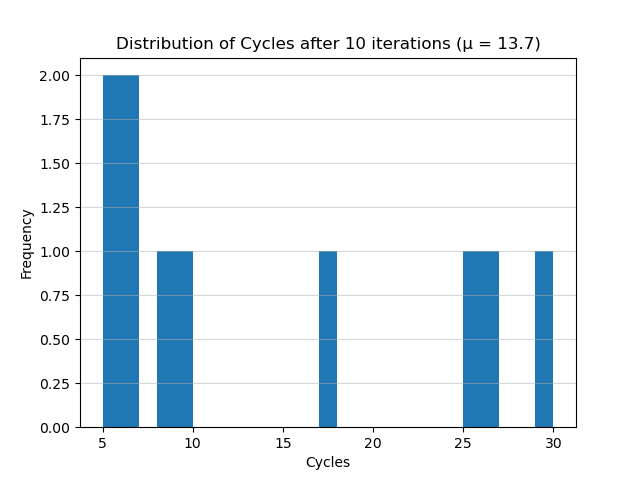
\includegraphics[width=\textwidth]{10.png}
  \caption{10 games}
  \label{fig:10}
\end{subfigure}%
\begin{subfigure}{.4\textwidth}
  \centering
  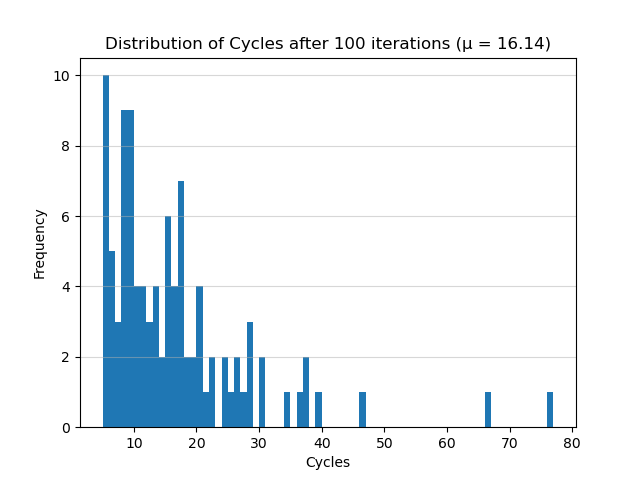
\includegraphics[width=\textwidth]{100.png}
  \caption{100 games}
\end{subfigure}
\caption{Plots of the distribution of cycles after simulating various numbers of games}
\label{fig:dist}
\end{figure}

\begin{figure}[H]
\centering
\begin{subfigure}{.5\textwidth}
  \centering
  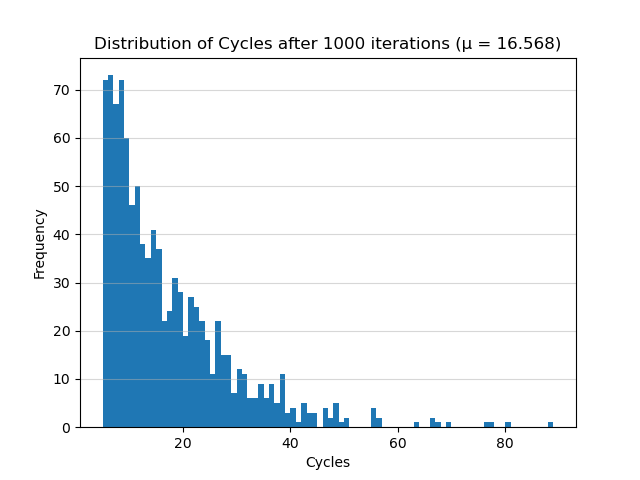
\includegraphics[width=\textwidth]{1000.png}
  \caption{1000 games}
\end{subfigure}%
\begin{subfigure}{.5\textwidth}
  \centering
  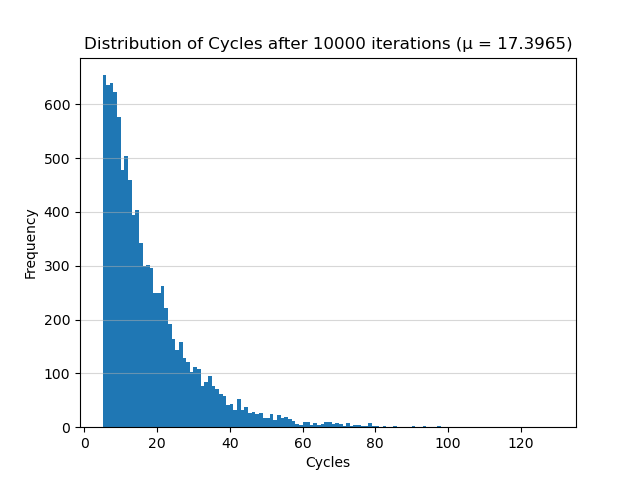
\includegraphics[width=\textwidth]{10000.png}
  \caption{10000 games}
  \label{fig:10000}
\end{subfigure}
\caption{Plots of the distribution of cycles after simulating various numbers of games}
\label{fig:dist}
\end{figure}

\begin{figure}[H]
\centering
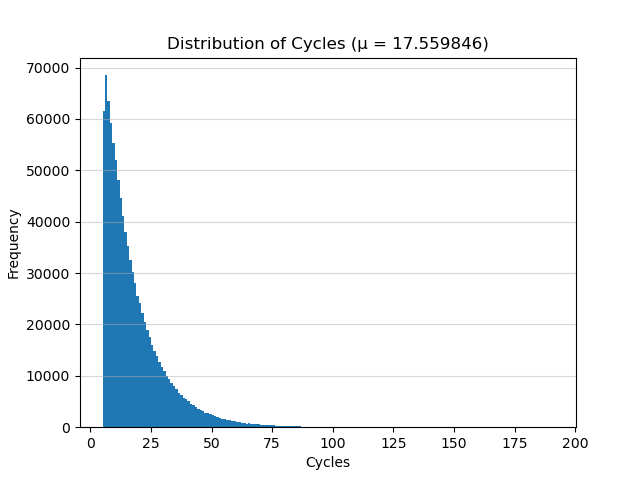
\includegraphics[width=.75\textwidth]{1000000.png}
\caption{Plots of the distribution of cycles after simulating 1,000,000 games}
\label{fig:1000000}
\end{figure}

It can be noted from these figures that the lowest number of cycles is 5 cycles. This is intuitive, since the players start with 4 coins, and would have to roll a 4, 5, or 6 five times in a row to lose the game in the least number of rolls. It can also be seen that the distribution of cycles becomes highly right-skewed as the number of games played increases. It is also worth noting that although the distribution looks like an exponential distribution, that is not so, as a property of the exponential distribution is that it is constantly decreasing, whereas it can be seen in Figure \ref{fig:1000000} that the frequency of `5 cycles' is lower than `6 cycles'.

To find the expected value of the distribution, the mean of the distribution of cycles was found. The movement of the mean over 1,000,000 games can be seen in Figure \ref{fig:mean}. It can be seen in this plot that the mean of the distribution eventually balances around 17.5603 cycles. Thus, it can be said that the expected value of the number of cycles of the ``Coins in a Pot" game is 17.5603 cycles. With access to more computational power, many more simulations may be run, which will bring the estimate of the expected value closer to the actual expected value.

\begin{figure}[H]
\centering
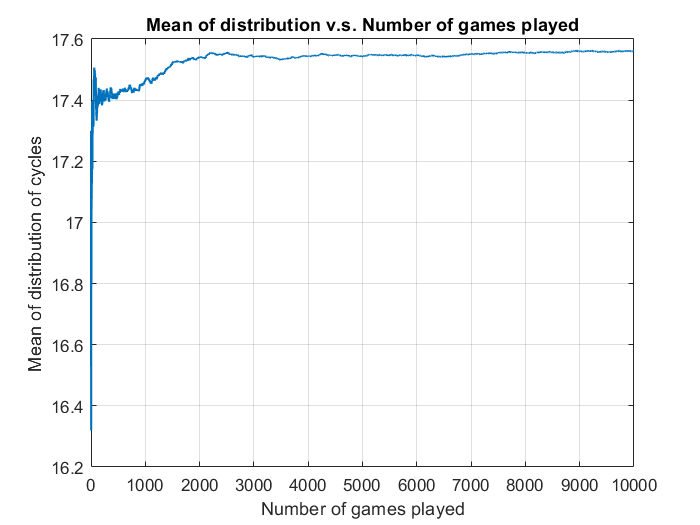
\includegraphics[width=.75\textwidth]{mean.png}
\caption{Mean of the distribution of cycles over 1,000,000 simulations}
\label{fig:mean}
\end{figure}


\section{Conclusions}

For this project, the expected value and distribution of the simple ``Coins in a Pot" game was found using simulation. Code was written in Python following the rules of the game, and was executed many times. As the number of repetitions increased, the statistics began to converge to certain values, which is consistent with the Law of Large Numbers.

Although the ``Coins in a Pot" game is seemingly simple, calculating its expected value by hand is a very arduous task. It is possible to find the expected value through first-step analysis, but, although this game is much simpler than a game such as Blackjack, the equation would grow rapidly and the number of terms in the equation would quickly become unmanageable. In more complicated games with more outcomes, finding the expected value would be unfeasible. In such cases, it is simpler to write code that accurately simulates a game, run the simulation millions of times, and record statistics of interest. Through this project, the importance of simulations for statistical analysis was revealed.



\appendix
\chapter{Python Code}
\label{pythoncode}
%{\large Python Code:}
\inputminted[linenos=true, breaklines=true, breakanywhere=true, fontsize=\footnotesize]{python}{../dice-game.py}

\end{document}

